\documentclass[10pt,a4paper]{article}
\usepackage[top=19mm,bottom=25.4mm,left=16mm,right=16mm]{geometry}
\usepackage{fontspec,graphicx,amsmath,amssymb,multicol,booktabs,array,tabularx}
\usepackage[hidelinks]{hyperref}
\setmainfont{Times New Roman}
\setlength{\columnsep}{6mm}
\setlength{\parindent}{0pt}
\setlength{\parskip}{3pt}
\setlength{\multicolsep}{4pt}
\setlength{\abovedisplayskip}{4pt}
\setlength{\belowdisplayskip}{4pt}
\pagestyle{empty}
\makeatletter
\renewcommand{\section}{\@startsection{section}{1}{0pt}{5pt}{2pt}{\normalfont\normalsize\bfseries}}
\makeatother
\newcommand{\sect}[1]{\section*{#1}}
\usepackage{xepersian}
\settextfont{B Nazanin}
\setlatintextfont{Times New Roman}
\begin{document}
\begin{center}
\includegraphics[width=\textwidth]{baic2026_header.png}\par\vspace{4pt}
{\fontsize{14}{17}\selectfont\bfseries انتخاب ویژگی با بودجه سخت و تعمیر مبتنی بر اطلاعات متقابل بازنمونه‌گیری‌شده در \lr{EHOA}}\par
امیررضا غفاریان\par
دانشجوی کارشناسی ارشد، دانشگاه آزاد اسلامی\end{center}
\textbf{چکیده. } تعمیر بودجه سخت در \lr{EHOA} را با سودمندی اطلاعات متقابل محلی هر تقسیم و جایگذاری، استانداردسازی و \lr{SMOTE} روی ستون‌های منتخب ارزیابی می‌کنیم. تحلیل اصلی پنج‌بذری شامل ۷۵۰ اجرا روی ده دیتاست است و برای هر روش/دیتاست پانزده ماسک نهایی وابسته دارد. در گسترش منتشرشده پیش از اجرا، طرح کامل انتهایی ۲×۲×۲ بودجه/\lr{R/lambda} روی ده دیتاست، ۲۴۰ اجرا و بررسی جست‌وجوی ۱۶ کوه‌پیما و ۲۰ تکرار، ۱۵۰ اجرا دارد. با حساسیت پزشکی قبلی، ۱۴۶۴ اجرای پایپ‌لاین مستقل موجود است. \lr{Steel} با ۲۷ پیش‌بین و هفت کلاس و ضبط‌های \lr{Parkinson} با تقسیم مستقل در سطح پیشوند فرد در هر دو سطح اجرا شدند. تعمیر بازنمونه‌گیری‌شده دقت متوازن \lr{0.7932}، نسبت هزینه \lr{0.2774} و پایداری نوگوئیرا \lr{0.2241} دارد؛ \lr{p} فریدمن دقت متوازن \lr{0.14237} است. مقایسه‌های زوجی اصلاح‌شده، تفسیر را محدود می‌کنند. همه خروجی‌های مقید بودجه را رعایت کردند. مخزن عمومی کد، انتساب داده عمومی، ثبت نسخه پروتکل و نتایج ممیزی‌شده را دارد. هزینه مصنوعی، هویت بالینی تأییدنشده و نبود داده بالینی بیرونی مستقل، مانع ادعای بالینی یا پولی‌اند. گسترش با اطلاع از نتایج قبلی طراحی شد و ثبت پیشینی گذشته نیست.

\textbf{کلیدواژه‌ها. } انتخاب ویژگی، بودجه سخت، اطلاعات متقابل بازنمونه‌گیری‌شده، پایداری زیرمجموعه
\begin{multicols}{2}\raggedcolumns
\sect{۱  مسئله و سهم پژوهش}
زیرمجموعه کوچک الزاماً کم‌هزینه نیست؛ هزینه کسب ویژگی‌ها می‌تواند متفاوت باشد. انتخاب با بودجه سخت، مجموع هزینه ویژگی‌های منتخب را محدود می‌کند \lr{[1].} پایداری زیرمجموعه، تغییر انتخاب ویژگی در نمونه‌های آموزش و جست‌وجوی تصادفی را می‌سنجد؛ این مفهوم با ثبات دقت یا همگرایی متفاوت است \lr{[2].} این تمایز برای تفسیر مجموعه اندازه‌گیری‌های زیست‌پزشکی اهمیت دارد.

انتخاب ویژگی پزشکی در تصویربرداری، سیگنال و داده مولکولی کاربرد دارد \lr{[3].} قدرت تفکیک پیش‌بینی، تکرارپذیری هویت ویژگی و بار کسب اندازه‌گیری، هدف‌های جداگانه‌اند. توصیفگرهای هم‌بسته می‌توانند جای یکدیگر را بگیرند؛ بنابراین تغییر ماسک الزاماً به معنای پیش‌بینی ضعیف نیست و تکرار ماسک نیز اعتبار زیست‌نشانگر را ثابت نمی‌کند. به همین دلیل، دقت متوازن، هزینه و پایداری تصحیح‌شده نسبت به شانس را هم‌زمان گزارش می‌کنیم.

جست‌وجوی \lr{EHOA} را حفظ می‌کنیم \lr{[4]} و نسخه نامقید را با چهار تعمیر در پایپ‌لاین ارزیابی یکسان روی ابعاد منتخب مقایسه می‌کنیم. میان نسخه‌های مقید، فقط سودمندی تعمیر متفاوت است. پیاده‌سازی \lr{FoldSafeEHOA} سودمندی محلی هر تقسیم و آموزش مختص هر کاندید را اجرا می‌کند؛ این نتایج تازه از پروتکل آرشیوی \lr{CostStableEHOA} جدا هستند. سهم پژوهش، مقایسه کنترل‌شده و قابل‌ممیزی است، نه خانواده بهینه‌سازی تازه.

\sect{۲  مطالعات مرتبط}
شاخص پایداری ممکن است انتخاب‌های تکرارپذیر اما کم‌ارزش را مطلوب نشان دهد؛ پایداری وزن‌دار با اهمیت ویژگی به این مسئله می‌پردازد \lr{[5].} انتخاب پزشکی با ریسک جریمه‌شده \lr{[6]}، کسب ترتیبی ویژگی \lr{[7]} و هزینه گروهی با ویژگی سایه \lr{[8]} مسائل مرتبط ولی متفاوتی‌اند. جدول ۱ تفاوت‌ها را نشان می‌دهد. \lr{NR} یعنی گزارش نشده در منبع بررسی‌شده؛ نتایج عددی این مطالعات با پروتکل حاضر مستقیماً مقایسه نمی‌شوند.

\par\vspace{3pt}\begin{minipage}{\linewidth}{\footnotesize جدول ۱. مقایسه مطالعات؛ جزئیات پروتکل در پیوست آمده است.\par}
\begin{latin}
{\fontsize{6.8}{8.3}\selectfont\setlength{\tabcolsep}{2pt}\renewcommand{\arraystretch}{1.1}
\begin{tabularx}{\linewidth}{>{\hsize=1.0000\hsize\raggedright\arraybackslash}X>{\hsize=1.0000\hsize\raggedright\arraybackslash}X>{\hsize=1.0000\hsize\raggedright\arraybackslash}X>{\hsize=1.0000\hsize\raggedright\arraybackslash}X>{\hsize=1.0000\hsize\raggedright\arraybackslash}X>{\hsize=1.0000\hsize\raggedright\arraybackslash}X}\toprule
Study & Budget & Costs & Stability & Evaluation & Difference\\\midrule
Jagdhuber [1] & Yes & Additive & NR & Simulation & Feasible GA\\
Nogueira [2] & NR & NR & Chance-corrected & Resampling & Metric\\
Hamer [5] & NR & NR & Importance-weighted & Resampling & Metric limits\\
Klonecki [6] & Yes & Feature / proxy & NR & Medical data & Penalized ERM\\
Valancius [7] & NR & Sequential & NR & AFA benchmarks & Patient-wise policy\\
Klonecki [8] & Yes & Grouped & NR & MIMIC & Shadow stopping\\
This work & Yes & Synthetic additive & Nogueira & 5 x 3 outer & MI/cost repair\\
\bottomrule\end{tabularx}}
\end{latin}
\end{minipage}\par\vspace{3pt}
انتخاب پایدار کلاسیک، انتخاب‌های تکرارشده در زیرنمونه‌ها را تجمیع می‌کند و با فرض‌ها و آستانه‌های مشخص، انتخاب کاذب را کنترل می‌کند \lr{[9,10].} چهار بازنمونه اطلاعات متقابل در روش حاضر، صرفاً سودمندی حذف را پیش از جست‌وجوی پوششی برآورد می‌کنند. احتمال انتخاب تکرارشده را آستانه‌گذاری نمی‌کنیم و تضمین کنترل خطای آن روش‌ها به این تعمیر منتقل نمی‌شود. شاخص نوگوئیرا ماسک‌های نهایی را ارزیابی می‌کند \lr{[2]} و تابع برازندگی بهینه‌شده نیست. کسب فعال \lr{[7]} اندازه‌گیری را برای هر نمونه به‌صورت متوالی انتخاب می‌کند؛ تعمیر حاضر زیرمجموعه ثابت و شدنی برمی‌گرداند.

\sect{۳  \lr{EHOA} پیاده‌سازی‌شده}
هر عضو جمعیت، موقعیت پیوسته \lr{x} و سرعت \lr{v} دارد؛ ماسک دودویی \lr{z} ویژگی‌ها را انتخاب می‌کند. مقداردهی اولیه از دنباله \lr{tent} با مقدار آغازین \lr{0.7} و پارامتر \lr{0.4} در بازه \lr{[-6,6]} استفاده می‌کند. سرعت اولیه در \lr{[-1.2,1.2]} یکنواخت است. به‌روزرسانی پیاده‌سازی در تکرار \lr{t} از \lr{T=10} چنین است:

\begin{latin}\begin{equation}\begin{gathered}\begin{aligned}v_i\leftarrow\operatorname{clip}_{[-12,12]}\big(&w_t v_i+SF_t[2r_1(p_i-x_i)\\&+2r_2(g-x_i)]\big)\end{aligned}\end{gathered}\end{equation}\end{latin}
\begin{latin}\begin{equation}\begin{gathered}\begin{gathered}x_i\leftarrow\operatorname{clip}_{[-6,6]}(x_i+v_i)\\w_t=0.9-0.5t/T,\quad SF_t=3-2t/T\end{gathered}\end{gathered}\end{equation}\end{latin}
در این روابط \lr{p\_i} و \lr{g} بهترین موقعیت پیوسته فردی و سراسری‌اند؛ \lr{r\_1} و \lr{r\_2} برای هر ویژگی مستقل و یکنواخت‌اند. احتمال انتخاب از سیگموئید \lr{1/(1+exp(-x\_j))} می‌آید. ماسک نمونه‌گیری‌شده تهی، ویژگی دارای بیشترین احتمال را بازمی‌گرداند. کد، رهبرهای پیوسته را از ماسک تعمیرشده جدا نگه می‌دارد، برازندگی ماسک تکراری را ذخیره می‌کند و پس از ده تکرار بدون توقف زودهنگام پایان می‌یابد.

\sect{۴  تعمیر بودجه محلی و پایداری}
هزینه‌ها واحدهای مصنوعی مثبت و جمع‌پذیرند و با بذر \lr{1000+D} از \lr{lognormal(0,0.7)} تولید می‌شوند. بودجه اصلی \lr{B=0.30 sum(c)} است؛ حساسیت \lr{0.15} و \lr{0.50} نیز بررسی شد. هزینه از برچسب مستقل است و پول واقعی نیست. هر ماسک مقید ناتهی باید \lr{sum(z\_j c\_j)<=B} را رعایت کند. کسب مشترک اندازه‌گیری به مدل هزینه گروهی متفاوت نیاز دارد \lr{[6,8].}

\begin{latin}\begin{equation}\begin{gathered}u_j=\max(0,\overline I_j-\lambda s_j),\quad q_j=u_j/c_j\end{gathered}\end{equation}\end{latin}
در هر تقسیم درونی، \lr{MI} فقط روی ردیف‌های آموزش همان تقسیم پس از جایگذاری برازش می‌شود. چهار بازنمونه درون‌کلاسی، \lr{ceil(0.8 n\_class)} ردیف با جایگذاری می‌گیرند؛ حداقل دو ردیف. برآوردگر پیوسته–گسسته سه همسایه دارد \lr{[11]}؛ در \lr{Dermatology}، ۳۳ ورودی درجه‌ای/گسسته و سن پیوسته در نظر گرفته شدند. واحد \lr{MI} نات و \lr{s\_j} انحراف معیار نمونه‌ای است. \lr{Lambda=1} سودمندی محافظه‌کارانه می‌دهد، نه کران اطمینان کالیبره‌شده؛ تقسیم بر \lr{sqrt(R)} نداریم. سودمندی آموزش بیرونی جداست و برای تعمیر کاندیدهای اعتبارسنجی درونی استفاده نمی‌شود.

\par\vspace{3pt}\begin{minipage}{\linewidth}{\footnotesize جدول ۲. هر چهار تعمیر، قاعده حذف یکسان دارند.\par}
\begin{latin}
{\fontsize{6.8}{8.3}\selectfont\setlength{\tabcolsep}{2pt}\renewcommand{\arraystretch}{1.1}
\begin{tabularx}{\linewidth}{>{\hsize=1.0000\hsize\raggedright\arraybackslash}X>{\hsize=1.0000\hsize\raggedright\arraybackslash}X>{\hsize=1.0000\hsize\raggedright\arraybackslash}X}\toprule
Repair & Utility u\_j & Meaning\\\midrule
Random/cost & U(0,1), fixed per training fold & Not uniform deletion\\
Cheapest & 1 & Largest cost first\\
MI/cost & Single-sample MI & Relevance per cost\\
Resampled/cost & max(0, mean MI - SD) & Conservative heuristic\\
\bottomrule\end{tabularx}}
\end{latin}
\end{minipage}\par\vspace{3pt}
جست‌وجو ماسک خام را نمونه‌گیری می‌کند. هر تقسیم درونی کاندید را با سودمندی آموزش خودش تعمیر می‌کند؛ سپس جایگذاری، استانداردسازی و \lr{SMOTE} فقط روی ستون‌های منتخب آموزش برازش می‌شوند \lr{[12].} ردیف اعتبارسنجی فقط تبدیل و پیش‌بینی می‌شود. برازندگی میانگین دقت معمولی و اندازه منتخب در سه تقسیم مستقل تعمیرشده است. کاندید خام برنده در پایان با سودمندی آموزش بیرونی تعمیر می‌شود؛ ماسک درونی و نهایی می‌توانند متفاوت باشند. طبقه‌بند بیرونی فقط روی ستون‌های منتخب نهایی دوباره برازش می‌شود. کل روش انتخاب و تعمیر ارزیابی می‌شود، نه یک ماسک ثابت مشترک میان همه تقسیم‌های درونی \lr{[13].}

\begin{latin}\begin{equation}\begin{gathered}\begin{gathered}F(z)=\frac13\sum_{f=1}^3F_f(z)\\F_f(z)=0.99(1-Acc_f)+0.01k_f/D\end{gathered}\end{gathered}\end{equation}\end{latin}
تا زمان عبور از بودجه، ویژگی فعال با کمترین سودمندی به هزینه حذف می‌شود. تک‌ویژگی غیرقابل‌خرید پاک می‌شود؛ ماسک تهی، ویژگی قابل‌خرید با بیشترین نسبت را بازیابی می‌کند. مثبت‌بودن هزینه و حذف متناهی، در صورت وجود یک ویژگی قابل‌خرید، شدنی‌بودن را تضمین می‌کنند؛ این شرط بررسی شد. این تضمین مربوط به بودجه است، نه پیش‌بینی بهینه. \lr{MI} همچنان حاشیه‌ای است و ممکن است تعامل یا افزونگی را نبیند.

\begin{latin}\begin{equation}\begin{gathered}\Phi=\operatorname{clip}_{[-1,1]}\left(1-\frac{\frac M{M-1}\frac1D\sum_j p_j(1-p_j)}{(\bar k/D)(1-\bar k/D)}\right)\end{gathered}\end{equation}\end{latin}
پایداری نوگوئیرا \lr{[2]} از \lr{M=15} ماسک نهایی هر دیتاست/تنظیم، فراوانی انتخاب \lr{p\_j} و میانگین اندازه استفاده می‌کند. ماسک‌های کامل/تهی یکسان در کد مقدار یک دارند. آموزش ماسک‌ها هم‌پوشانی دارد و مستقل نیستند؛ مقدار پایداری تکرارشده، پانزده مشاهده مستقل نیست. جاکارد شاخص مکمل هم‌پوشانی بدون تصحیح شانس است.

\sect{۵  دیتاست‌ها و اصلاح منبع}
\par\vspace{3pt}\begin{minipage}{\linewidth}{\footnotesize جدول ۳. مشخصات داده اجرای تازه؛ \lr{U} شناسه مستقیم دیتاست \lr{UCI} است.\par}
\begin{latin}
{\fontsize{6.8}{8.3}\selectfont\setlength{\tabcolsep}{2pt}\renewcommand{\arraystretch}{1.1}
\begin{tabularx}{\linewidth}{>{\hsize=1.8947\hsize\raggedright\arraybackslash}X>{\hsize=0.5684\hsize\raggedright\arraybackslash}X>{\hsize=0.3789\hsize\raggedright\arraybackslash}X>{\hsize=0.3789\hsize\raggedright\arraybackslash}X>{\hsize=2.1474\hsize\raggedright\arraybackslash}X>{\hsize=0.6316\hsize\raggedright\arraybackslash}X}\toprule
Dataset & N & D & K & Class counts & Source\\\midrule
Breast Cancer & 569 & 30 & 2 & 212/ 357 & U17\\
Wine & 178 & 13 & 3 & 59/ 71/ 48 & U109\\
Ionosphere & 350 & 34 & 2 & 125/ 225 & U52\\
Sonar & 208 & 60 & 2 & 111/ 97 & U151\\
Dermatology & 366 & 34 & 6 & 112/ 61/ 72/ 49/ 52/ 20 & U33\\
Spambase & 4210 & 57 & 2 & 2531/ 1679 & U94\\
Parkinson (grouped) & 195 & 22 & 2 & 48/ 147 & U174\\
Hill Valley & 1212 & 100 & 2 & 606/ 606 & U166\\
Steel (corrected) & 1941 & 27 & 7 & 158/ 190/ 391/ 72/ 55/ 402/ 673 & U198\\
Madelon & 2600 & 500 & 2 & 1300/ 1300 & U171\\
\bottomrule\end{tabularx}}
\end{latin}
\end{minipage}\par\vspace{3pt}
تکرار دقیق \lr{(X,y)} حذف شد: \lr{Ionosphere} شامل ۳۵۰ و \lr{Spambase} شامل ۴۲۱۰ ردیف است. شش نشانگر هدف از ورودی \lr{Steel} حذف و هفت کلاس عیب بازسازی شد. ضبط‌های \lr{Parkinson} به فایل عددی \lr{UCI} تطبیق یافتند و ۳۲ پیشوند فرد در تقسیم گروهی درونی و بیرونی استفاده شدند. متن \lr{UCI} تعداد ۳۱ فرد را می‌گوید؛ هویت بالینی گروه‌ها هنوز تأیید مستقل ندارد. داده خام و نتایج قبلی حفظ شدند.

\sect{۶  پروتکل تازه و تحلیل آماری}
مطالعه مستقل اولیه سه بذر داشت؛ دو بذر اضافه، پنج بذر \lr{72001-72005}، سه تقسیم بیرونی و ۷۵۰ اجرای اصلی برای ده دیتاست و پنج روش می‌دهند. پروتکل گسترش و هش کد در ثبت \lr{GitHub} با شناسه \lr{72c87b6} پیش از ۶۹۰ اجرای آن منتشر شدند: ۳۰۰ تکرار بذری، ۲۴۰ اجرای فاکتوریل کامل و ۱۵۰ اجرای جست‌وجوی بزرگ‌تر. نتایج قبلی شناخته‌شده بودند. این نسخه‌گذاری آینده‌نگر است، نه ثبت رسمی مستقل یا ثبت آزمایش گذشته. سودمندی درونی فقط برچسب آموزش را می‌بیند و آزمون بیرونی برای انتخاب تنظیم برنده استفاده نمی‌شود.

\par\vspace{3pt}\begin{minipage}{\linewidth}{\footnotesize جدول ۴. تنظیم‌های واقعی تثبیت‌شده.\par}
\begin{latin}
{\fontsize{6.8}{8.3}\selectfont\setlength{\tabcolsep}{2pt}\renewcommand{\arraystretch}{1.1}
\begin{tabularx}{\linewidth}{>{\hsize=1.0000\hsize\raggedright\arraybackslash}X>{\hsize=1.0000\hsize\raggedright\arraybackslash}X}\toprule
Parameter & Value\\\midrule
Population / iterations & Primary 8/10; search study 16/20\\
Position / velocity clip & [-6,6] / [-12,12]\\
Tent / sweep / inertia & 0.7,p=0.4 / 3 to 1 / 0.9 to 0.4\\
c1,c2 / alpha & 2,2 / 0.99\\
Outer / inner folds & 3 / 3; Parkinson grouped\\
Outer seeds & 72001-72005\\
Selector seed & outer seed + fold index x 100003\\
Primary R / fraction / lambda & 4 / 0.8 with replacement / 1\\
Sensitivity R / lambda & Factorial 4,8 / 0,2; earlier OFAT 4,8,16 / 0,1,2\\
Cost / budgets & lognormal(0,0.7) / 15,30,50\%\\
Classifier & 5-NN; uniform; Euclidean\\
Imputation / scale / SMOTE & Training-selected columns only\\
Timing & Includes utility and final classification\\
\bottomrule\end{tabularx}}
\end{latin}
\end{minipage}\par\vspace{3pt}
هر دیتاست یک میانگین هر روش و یک برآورد پایداری می‌دهد \lr{[14].} فریدمن از ده بلوک دیتاست، تصحیح تساوی و \lr{df=4} استفاده می‌کند. ویلکاکسون دوطرفه، تعمیر بازنمونه‌گیری‌شده را با چهار کنترل مقایسه می‌کند؛ هولم هم درون هر معیار و هم روی همه ۲۴ مقایسه اعمال شد. شش آزمون کلی نیز اصلاح شدند. فاصله‌های بازنمونه‌گیری دیتاستی با ۲۰٬۰۰۰ تکرار و بذر \lr{20261012}، توصیفی و بدون اصلاح‌اند. پانزده ماسک وابسته، تکرارهای مستقل محسوب نمی‌شوند.

\sect{۷  نتایج و حساسیت}
\par\vspace{3pt}\begin{minipage}{\linewidth}{\footnotesize جدول ۵. میانگین هم‌وزن ده دیتاست؛ \lr{V} عبور از بودجه است.\par}
\begin{latin}
{\fontsize{6.8}{8.3}\selectfont\setlength{\tabcolsep}{2pt}\renewcommand{\arraystretch}{1.1}
\begin{tabularx}{\linewidth}{>{\hsize=1.0000\hsize\raggedright\arraybackslash}X>{\hsize=1.0000\hsize\raggedright\arraybackslash}X>{\hsize=1.0000\hsize\raggedright\arraybackslash}X>{\hsize=1.0000\hsize\raggedright\arraybackslash}X>{\hsize=1.0000\hsize\raggedright\arraybackslash}X>{\hsize=1.0000\hsize\raggedright\arraybackslash}X}\toprule
Method & BA & Cost ratio & Size & Stability & V\\\midrule
EHOA & 0.7946 & 0.4947 & 42.84 & 0.1036 & 145/150\\
Random/cost & 0.7814 & 0.2724 & 31.59 & 0.1217 & 0/150\\
Cheapest & 0.7944 & 0.2765 & 35.05 & 0.2476 & 0/150\\
MI/cost & 0.7949 & 0.2787 & 27.31 & 0.2203 & 0/150\\
Resamp./cost & 0.7932 & 0.2774 & 31.24 & 0.2241 & 0/150\\
\bottomrule\end{tabularx}}
\end{latin}
\end{minipage}\par\vspace{3pt}
\par\vspace{3pt}\begin{minipage}{\linewidth}{\footnotesize جدول ۶. فریدمن و رتبه میانگین به ترتیب \lr{E/R/C/M/S}؛ رتبه کمتر بهتر است.\par}
\begin{latin}
{\fontsize{6.8}{8.3}\selectfont\setlength{\tabcolsep}{2pt}\renewcommand{\arraystretch}{1.1}
\begin{tabularx}{\linewidth}{>{\hsize=1.0000\hsize\raggedright\arraybackslash}X>{\hsize=1.0000\hsize\raggedright\arraybackslash}X>{\hsize=1.0000\hsize\raggedright\arraybackslash}X>{\hsize=1.0000\hsize\raggedright\arraybackslash}X>{\hsize=1.0000\hsize\raggedright\arraybackslash}X>{\hsize=1.0000\hsize\raggedright\arraybackslash}X>{\hsize=1.0000\hsize\raggedright\arraybackslash}X>{\hsize=1.0000\hsize\raggedright\arraybackslash}X}\toprule
Metric & Chi2 & p & E & R & C & M & S\\\midrule
BA & 6.8800 & 0.14237 & 2.50 & 4.10 & 2.60 & 2.70 & 3.10\\
Cost & 21.2000 & 0.00029 & 5.00 & 2.20 & 2.60 & 2.90 & 2.30\\
Size & 29.1313 & <0.00001 & 5.00 & 1.85 & 3.55 & 1.75 & 2.85\\
Stability & 29.6800 & <0.00001 & 4.70 & 4.20 & 1.60 & 2.20 & 2.30\\
\bottomrule\end{tabularx}}
\end{latin}
\end{minipage}\par\vspace{3pt}
دلتای تعمیر بازنمونه‌گیری‌شده نسبت به \lr{EHOA} برای \lr{BA} برابر \lr{-0.00141} است؛ \lr{W=22}، هولم درون معیار \lr{1.00000}، اثر رتبه‌ای \lr{r=-0.200} و فاصله توصیفی ۹۵ درصد \lr{[-0.01024,0.00799].} دلتای پایداری \lr{+0.12045} است؛ هولم درون معیار \lr{0.00781} و همه ۲۴ مقایسه \lr{0.04688.} دلتای هزینه \lr{-0.21732} است؛ هولم درون معیار \lr{0.00781} و همه ۲۴ مقایسه \lr{0.04688.} این مقایسه شامل اعمال بودجه بر \lr{EHOA} نامقید است و اثر بازنمونه‌گیری را به‌تنهایی جدا نمی‌کند. عدم معناداری، هم‌ارزی را ثابت نمی‌کند.

طرح کامل ۲×۲×۲، بودجه \lr{0.15/0.50}، \lr{R=4/8} و \lr{lambda=0/2} را روی هر ده دیتاست ترکیب می‌کند. کنتراست متعامد، اثر اصلی، تعامل دوتایی و سه‌تایی انتهایی را می‌سنجد. هر خانه یک بذر و سه تقسیم بیرونی دارد؛ بنابراین تعامل‌ها توصیفی‌اند و کل فضای پیوسته پارامتر را پوشش نمی‌دهند. بررسی جست‌وجوی بزرگ‌تر، ۱۶ کوه‌پیما و ۲۰ تکرار را با ۸ و ۱۰، روی بذر \lr{72001}، تقسیم‌های مشترک و هر پنج روش مقایسه می‌کند. همه تنظیم‌ها گزارش شدند و برنده‌ای از آزمون بیرونی انتخاب نشد.

تعمیر ارزان‌ترین میانگین پایداری بیشتری دارد \lr{(0.2476)} نسبت به تعمیر بازنمونه‌گیری‌شده \lr{(0.2241)}؛ دلتای زوجی \lr{-0.02347} و هولم درون معیار \lr{0.21094} است. بنابراین بازنمونه‌گیری برتری پایداری اصلاح‌شده نسبت به ارزان‌ترین یا تعمیر \lr{MI} تک‌نمونه‌ای ندارد. بهبود توصیفی نسبت به پایه نامقید، شاهد برتری بر جایگزین ساده‌تر شدنی نیست.

اثر انتهایی \lr{R=8} نسبت به \lr{R=4} بر \lr{BA}، با میانگین‌گیری روی بودجه و جریمه، \lr{+0.00786} و فاصله توصیفی \lr{[0.00154,0.01527]} است. جست‌وجوی بزرگ‌تر برازندگی درونی تعمیر بازنمونه‌گیری‌شده را \lr{-0.01554} تغییر می‌دهد؛ اما دلتای \lr{BA} بیرونی \lr{-0.00424} و فاصله \lr{[-0.02869,0.01940]} است. بنابراین برازندگی درونی بهتر، پیش‌بینی آزمون بهتر را ثابت نمی‌کند. فاصله‌ها کنتراست توصیفی بدون اصلاح‌اند و تنظیم اصلی را انتخاب نمی‌کنند.

\par\begin{minipage}{\linewidth}\centering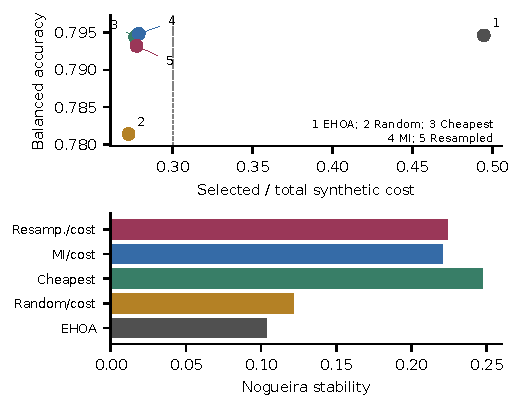
\includegraphics[width=\linewidth]{figures/eligible_comparison.pdf}\par{\footnotesize شکل ۱. میانگین ده دیتاست اجرای تازه؛ هزینه مصنوعی و پایداری توصیفی زیرمجموعه.\par}\end{minipage}\par
\sect{۸  مطالعه پزشکی و ارتباط با کنگره}
داده تشخیصی سرطان پستان شامل ۵۶۹ نمونه آسپیراسیون سوزن ظریف، ۲۱۲ بدخیم و ۳۵۷ خوش‌خیم، با ۳۰ توصیفگر تصویر هسته است \lr{[15].} جدول ۷ و شکل ۲، پانزده ماسک هر روش را نشان می‌دهند. شمارش، انتخاب محاسباتی را توصیف می‌کند، نه زیست‌نشانگر علّی. چند توصیفگر از یک کسب تصویر مشترک می‌آیند؛ هزینه مصنوعی جمع‌پذیر، صرفه‌جویی در قیمت نمونه‌برداری نیست. برچسب \lr{0} بدخیم و \lr{1} خوش‌خیم است؛ بازخوانی هر کلاس صریح گزارش شد.

\par\vspace{3pt}\begin{minipage}{\linewidth}{\footnotesize جدول ۷. سرطان پستان: پانزده اجرا هر روش.\par}
\begin{latin}
{\fontsize{6.8}{8.3}\selectfont\setlength{\tabcolsep}{2pt}\renewcommand{\arraystretch}{1.1}
\begin{tabularx}{\linewidth}{>{\hsize=1.0000\hsize\raggedright\arraybackslash}X>{\hsize=1.0000\hsize\raggedright\arraybackslash}X>{\hsize=1.0000\hsize\raggedright\arraybackslash}X>{\hsize=1.0000\hsize\raggedright\arraybackslash}X>{\hsize=1.0000\hsize\raggedright\arraybackslash}X>{\hsize=1.0000\hsize\raggedright\arraybackslash}X}\toprule
Method & BA & Mal. sens. & Ben. spec. & Cost & Stability\\\midrule
EHOA & 0.9512 & 0.9415 & 0.9608 & 0.5620 & 0.0727\\
Random/cost & 0.9382 & 0.9217 & 0.9546 & 0.2525 & 0.0988\\
Cheapest & 0.9519 & 0.9368 & 0.9669 & 0.2707 & 0.1975\\
MI/cost & 0.9517 & 0.9387 & 0.9647 & 0.2771 & 0.2046\\
Resamp./cost & 0.9493 & 0.9340 & 0.9647 & 0.2751 & 0.1757\\
\bottomrule\end{tabularx}}
\end{latin}
\end{minipage}\par\vspace{3pt}
\par\begin{minipage}{\linewidth}\centering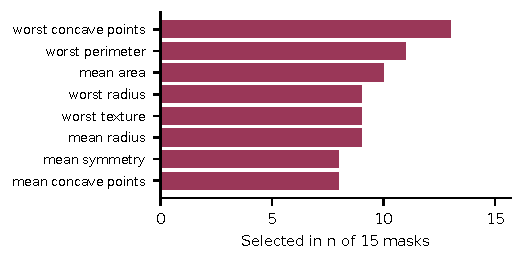
\includegraphics[width=\linewidth]{figures/breast_top_frequencies.pdf}\par{\footnotesize شکل ۲. شمار انتخاب هشت ویژگی پرتکرار در پانزده ماسک تعمیر بازنمونه‌گیری‌شده.\par}\end{minipage}\par
نزدیک‌ترین محور رسمی \lr{BAIC2026}، هوش مصنوعی، یادگیری ماشین و علم داده / سیستم‌های هوشمند تشخیص بیماری است \lr{(baic.um.ac.ir/fa/home/Content/12).} سهم پژوهش انتخاب محاسباتی مجموعه اندازه‌گیری است؛ سامانه تشخیصی معتبر بالینی یا سازوکار شناختی ادعا نمی‌کنیم.

\sect{۹  محدودیت‌ها و بازتولیدپذیری}
مطالعه اکنون پنج بذر اصلی، تعامل انتهایی روی ده دیتاست و پروفایل جست‌وجوی بزرگ‌تر دارد. با این حال، یک بذر در فاکتوریل و مقایسه جست‌وجو همه تغییرپذیری تصادفی را توصیف نمی‌کند؛ جست‌وجوی متناهی، همگرایی یا بهینه سراسری را ثابت نمی‌کند. \lr{MI} حاشیه‌ای و میانگین منهای \lr{SD} فاقد پوشش اطمینان یا کنترل انتخاب کاذب‌اند. هزینه مصنوعی است، هویت فرد به تأیید مستقل نیاز دارد و داده بالینی بیرونی موجود نیست. دسته‌های زمان‌سنجی هم‌زمانی متفاوت سه و شش پردازش دارند؛ مقایسه زمان، بنچمارک کنترل‌شده سرعت نیست.

مخزن عمومی \lr{github.com/Amirgh23/coststable-ehoa} کد، \lr{snapshot} عمومی با انتساب \lr{CC BY}، ثبت نسخه پروتکل، نتایج و ماسک‌ها را دارد. بسته محلی، پیش‌بینی هر ۱۴۶۴ اجرا، اندیس ردیف، سودمندی و ممیزی کاندید را نیز ارائه می‌کند. شناسه منبع \lr{Hill-Valley} از ۱۴۷ به ۱۶۶ اصلاح شد و داده عددی \lr{OpenML 1479} تغییر نکرد. دسته‌های اصلی و حساسیت قدیمی با نسخه خود حفظ شدند. دسترسی عمومی، مشکل دسترسی کد را رفع می‌کند؛ اعتبار بالینی یا ثبت پیشینی گذشته را ثابت نمی‌کند.

\sect{۱۰  نتیجه‌گیری}
پروتکل بازطراحی‌شده، کل پایپ‌لاین آموزش و تعمیر را با سودمندی محلی و بازنمونه‌گیری روی ابعاد منتخب ارزیابی می‌کند. همه ماسک‌های مقید شدنی‌اند. تفسیر باید براساس شواهد زوجی اصلاح‌شده و مقایسه با تعمیرهای ساده‌تر شدنی باشد. ادعای بالینی و پولی همچنان به هزینه واقعی گروهی و اعتبارسنجی بالینی مستقل نیاز دارد.

\sect{مراجع}
\begin{minipage}{\linewidth}{\fontsize{7}{8.2}\selectfont \begin{latin}[1] R. Jagdhuber, M. Lang, A. Stenzl, J. Neuhaus, and J. Rahnenführer, "Cost-Constrained feature selection in binary classification: adaptations for greedy forward selection and genetic algorithms," BMC Bioinformatics, vol. 21, art. 26, 2020. \url{https://doi.org/10.1186/s12859-020-3361-9}\end{latin}\par}\end{minipage}\par
\begin{minipage}{\linewidth}{\fontsize{7}{8.2}\selectfont \begin{latin}[2] S. Nogueira, K. Sechidis, and G. Brown, "On the Stability of Feature Selection Algorithms," Journal of Machine Learning Research, vol. 18, no. 174, pp. 1-54, 2018. \url{https://jmlr.org/papers/v18/17-514.html}\end{latin}\par}\end{minipage}\par
\begin{minipage}{\linewidth}{\fontsize{7}{8.2}\selectfont \begin{latin}[3] B. Remeseiro and V. Bolon-Canedo, "A review of feature selection methods in medical applications," Computers in Biology and Medicine, vol. 112, art. 103375, 2019. \url{https://doi.org/10.1016/j.compbiomed.2019.103375}\end{latin}\par}\end{minipage}\par
\begin{minipage}{\linewidth}{\fontsize{7}{8.2}\selectfont \begin{latin}[4] A. E. Hegazy, M. A. Makhlouf, O. A. M. Salem, and B. Hafiz, "An enhanced Hiking optimization algorithm for accurate and interpretable feature selection in medical data classification," Cluster Computing, vol. 29, art. 244, 2026. \url{https://doi.org/10.1007/s10586-026-05946-9}\end{latin}\par}\end{minipage}\par
\begin{minipage}{\linewidth}{\fontsize{7}{8.2}\selectfont \begin{latin}[5] V. Hamer and P. Dupont, "An Importance Weighted Feature Selection Stability Measure," Journal of Machine Learning Research, vol. 22, no. 116, pp. 1-57, 2021. \url{https://jmlr.org/papers/v22/20-366.html}\end{latin}\par}\end{minipage}\par
\begin{minipage}{\linewidth}{\fontsize{7}{8.2}\selectfont \begin{latin}[6] T. Klonecki and P. Teisseyre, "Feature selection under budget constraint in medical applications: analysis of penalized empirical risk minimization methods," Applied Intelligence, vol. 53, pp. 29943-29973, 2023. \url{https://doi.org/10.1007/s10489-023-05063-9}\end{latin}\par}\end{minipage}\par
\begin{minipage}{\linewidth}{\fontsize{7}{8.2}\selectfont \begin{latin}[7] M. Valancius, M. Lennon, and J. Oliva, "Acquisition Conditioned Oracle for Nongreedy Active Feature Acquisition," Proceedings of the 41st International Conference on Machine Learning, PMLR, vol. 235, pp. 48957-48975, 2024. \url{https://proceedings.mlr.press/v235/valancius24a.html}\end{latin}\par}\end{minipage}\par
\begin{minipage}{\linewidth}{\fontsize{7}{8.2}\selectfont \begin{latin}[8] T. Klonecki, P. Teisseyre, and J. Lee, "Cost-Constrained Multi-label Group Feature Selection Using Shadow Features," in Advances in Artificial Intelligence Research, PP-RAI 2025, Lecture Notes in Networks and Systems, vol. 1599, pp. 3-16, Springer, 2026. \url{https://doi.org/10.1007/978-3-032-04197-5_1}\end{latin}\par}\end{minipage}\par
\begin{minipage}{\linewidth}{\fontsize{7}{8.2}\selectfont \begin{latin}[9] N. Meinshausen and P. Buhlmann, "Stability selection," Journal of the Royal Statistical Society: Series B, vol. 72, no. 4, pp. 417-473, 2010. \url{https://doi.org/10.1111/j.1467-9868.2010.00740.x}\end{latin}\par}\end{minipage}\par
\begin{minipage}{\linewidth}{\fontsize{7}{8.2}\selectfont \begin{latin}[10] R. D. Shah and R. J. Samworth, "Variable selection with error control: another look at stability selection," Journal of the Royal Statistical Society: Series B, vol. 75, no. 1, pp. 55-80, 2013. \url{https://doi.org/10.1111/j.1467-9868.2011.01034.x}\end{latin}\par}\end{minipage}\par
\begin{minipage}{\linewidth}{\fontsize{7}{8.2}\selectfont \begin{latin}[11] B. C. Ross, "Mutual Information between Discrete and Continuous Data Sets," PLOS ONE, vol. 9, no. 2, art. e87357, 2014. \url{https://doi.org/10.1371/journal.pone.0087357}\end{latin}\par}\end{minipage}\par
\begin{minipage}{\linewidth}{\fontsize{7}{8.2}\selectfont \begin{latin}[12] N. V. Chawla, K. W. Bowyer, L. O. Hall, and W. P. Kegelmeyer, "SMOTE: Synthetic Minority Over-sampling Technique," Journal of Artificial Intelligence Research, vol. 16, pp. 321-357, 2002. \url{https://doi.org/10.1613/jair.953}\end{latin}\par}\end{minipage}\par
\begin{minipage}{\linewidth}{\fontsize{7}{8.2}\selectfont \begin{latin}[13] S. Varma and R. Simon, "Bias in error estimation when using cross-validation for model selection," BMC Bioinformatics, vol. 7, art. 91, 2006. \url{https://doi.org/10.1186/1471-2105-7-91}\end{latin}\par}\end{minipage}\par
\begin{minipage}{\linewidth}{\fontsize{7}{8.2}\selectfont \begin{latin}[14] J. Demšar, "Statistical Comparisons of Classifiers over Multiple Data Sets," Journal of Machine Learning Research, vol. 7, pp. 1-30, 2006. \url{https://jmlr.org/papers/v7/demsar06a.html}\end{latin}\par}\end{minipage}\par
\begin{minipage}{\linewidth}{\fontsize{7}{8.2}\selectfont \begin{latin}[15] W. Wolberg, O. Mangasarian, N. Street, and W. Street, "Breast Cancer Wisconsin (Diagnostic)," UCI Machine Learning Repository, 1993. \url{https://doi.org/10.24432/C5DW2B}\end{latin}\par}\end{minipage}\par
\end{multicols}
\end{document}